\documentclass[12pt,a4paper]{report}
\usepackage{amssymb,amsthm,amsmath,amscd}
\usepackage{latexsym}
\usepackage{enumerate}
\usepackage[german]{babel}
\usepackage{verbatim}
\usepackage[hyphens]{url}
\usepackage{hyperref}
\usepackage[utf8]{inputenc}
\usepackage{pdfpages}
\usepackage{graphicx}
\usepackage{csquotes}
\begin{document}
\begin{titlepage}
	\begin{center}

		\vspace*{1.0cm}
		\huge
		\textsc{\bf{PS Algorithmen für verteilte Systeme}}

		\vspace*{4.0cm}
		\textsc{
			\normalsize{eingereicht von} \\[0.5\baselineskip]
			{\large Baumgartner Dominik, Dafir Samy}
		}

		\vspace*{3.0cm}
		\textsc{
			\normalsize{Gruppe  1(16:00)}
		}

	\end{center}
\end{titlepage}

\section*{Aufgabe 14}
Sei $d$ = ($d_1\dots d_n$) eine Sequenz von n natürlichen Zahlen. Ein Graph $G = (V, E)$ mit $V = \{v_1,\dots, v_n\}$ hat Gradsequenz $d$, wenn für alle $i \in \{1,\dots, n\}$ gilt, dass Knoten $v_i$ Grad $d_i$ hat. Haben zwei Graphen mit der selben Gradsequenz den gleichen Durchmesser? Begründen Sie Ihre Antwort.
\\
\\
Antwort: Zwei Graphen mit der selben Gradsequenz haben nicht immer den gleichen Durchmesser. Dies lässt sich anhand eines einfachen Gegenbeispiels zeigen.\\
\\
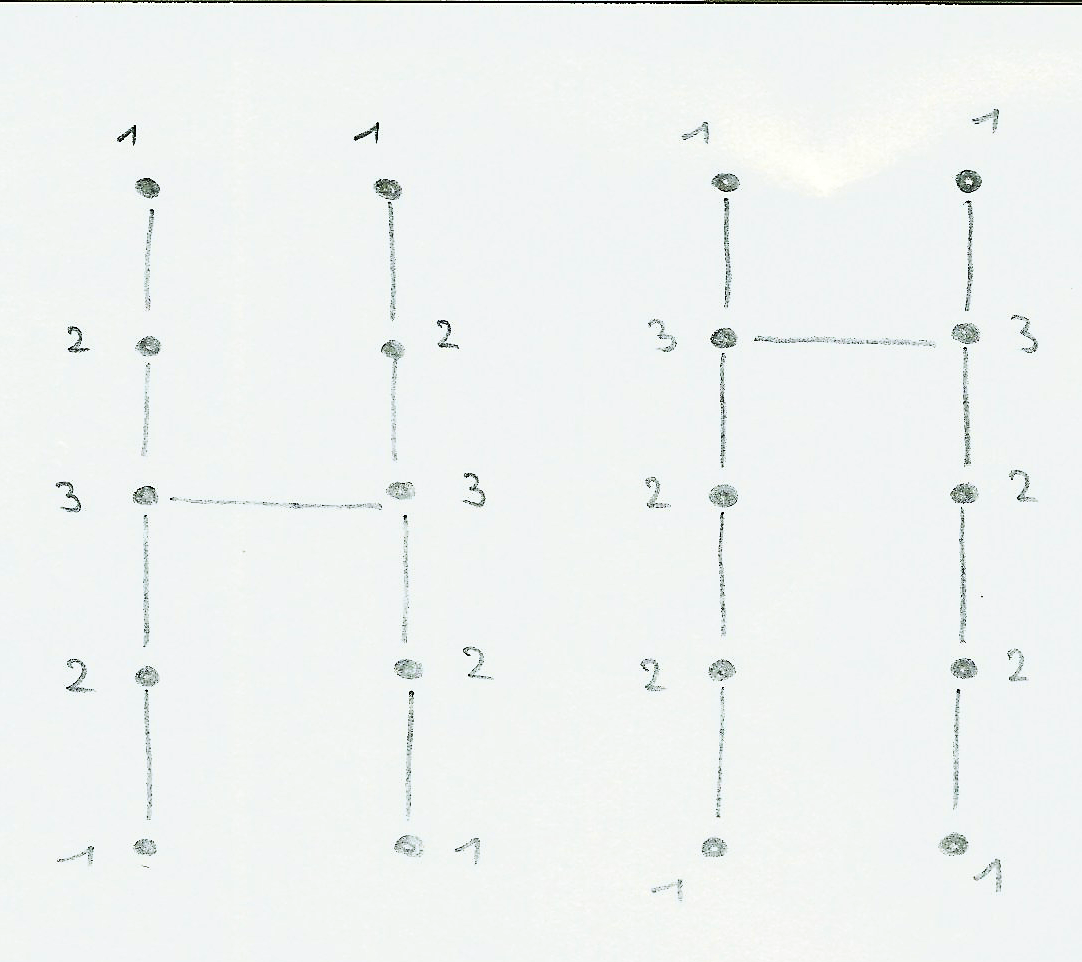
\includegraphics[height=8cm]{gegenbsp.png}
\\
\\
Beide Graphen haben die Gradsequenz $d$ = $(1,1,1,1,2,2,2,2,3,3)$.\\
Der Durchmesser des linken Graphen beträgt 5, der des rechten 7. Damit ist ein Gegenbeispiel gefunden und die Behauptung ist widerlegt.
Der Durchmesser ist der kürzeste Weg zwischen den am weitesten entfernten Knoten des Graphen, in unserem Fall also in beiden Graphen vom linken unteren zum rechten unteren Knoten mit Grad 1.
\end{document}
